% !TEX encoding = UTF-8 Unicode

\documentclass[a4paper]{article}

\usepackage{color}
\usepackage{url}
\usepackage[utf8]{inputenc} % make weird characters work
\usepackage{graphicx}
\usepackage[english,serbian]{babel}
\usepackage[unicode]{hyperref}
\usepackage{amsthm}
\usepackage{amssymb}
\usepackage{float}
\usepackage[graphicx]{realboxes}
\usepackage[font=small,labelfont=bf]{caption}
\usepackage{chngcntr}
\counterwithin{figure}{section}
\hypersetup{colorlinks,citecolor=green,filecolor=green,linkcolor=blue,urlcolor=blue}


\theoremstyle{plain}
\newtheorem{thm}{Teorema}[section] % reset theorem numbering for each chapter
\theoremstyle{definition}
\newtheorem{defn}[thm]{Definicija} % definition numbers are dependent on theorem numbers
\newtheorem{lem}[thm]{Lema} % lemma numbers are dependent on theorem
\newtheorem{exmp}[thm]{Primer} % same for example numbers


\begin{document}

\title{Procenjivanje minimalne povr\v{s}ine pravougaonih i konveksnih kontejnera za problem pakovanja konveksnih poligona koriste\'c{}i translacije\\  \small{Seminarski rad u okviru kursa\\Geometrijski algoritmi\\ Matematički fakultet}}

\author{\href{mailto:mi14042@matf.bg.ac.rs}{Ivan Ristovi\'c}}
\date{decembar 2018.}

\maketitle

\abstract{
    Algoritmi za efikasno pakovanje objekata imaju va\v{z}ne primene. Sam problem ima raznorazne varijante, od kojih su autori izabrali pakovanje konveksnih poligona u kontejner oblika pravougaonika pri \v{c}emu su dozvoljene samo translacije poligona. Autori predstavljaju algoritam vremenske slo\v{z}enosti $O(n\log{}n)$ za re\v{s}avanje datog problema. \v{S}tavi\v{s}e, autori dokazuju da je povr\v{s}ina dobijenog re\v{s}enja najvi\v{s}e $17.45$ puta ve\'c{}a od optimalne, \v{s}to je prvi poznati dokaz da se ovako te\v{s}ki NP-te\v{s}ki problemi uop\v{s}te mogu aproksimirati. Takodje, autori razmatraju problem pakovanje poligona u konveksne kontejnere povr\v{s}ine najvi\v{s}e $27$ puta ve\'c{}e od optimalne.
}

\tableofcontents

\newpage

\section{Uvod}
\label{sec:Uvod}

Problem efikasnog pakovanja objekata u kontejnere ima raznolike varijacije i ogromne primene od kojih \'c{}e par biti navedeno. Dvodimenzionalne verzije problema se javljaju u tzv. \emph{pakovanju u trake} \cite{paper} [12, 13, 5], gde se dati skup objekata pakuje u pravougaone trake fiksne \v{s}irine minimizuju\'c{}i \v{s}irinu trake. U tri dimenzije, problem se prirodno javlja u minimizaciji prostora prilikom transportovanja objekata.

Oblik objekata je od velikog uticaja na slo\v{z}enost problema. U dve dimenzije mo\v{z}emo razmatrati pravilne poligone, pravougaonike, proste ili konveksne poligone. Pritom, mora se specifikovati koje transformacije objekata su dozvoljene - da li ih je dozvoljeno rotirati ili samo translirati. 

Ve\'c{} su jednostavne varijante ovog problema NP-te\v{s}ke, recimo pakovanje skupa pravougaonika sa stranicama paralelnim koordinatnim osama koriste\'c{}i samo translacije, \v{s}to je pokazano u \cite{paper} [4] tako da se polinomijalni algoritmi mogu konstruisati samo ukoliko je broj objekata konstantan \cite{paper} [1, 2, 14, 3, 8, 9, 10, 7]. Stoga su konstruisani razni algoritmi za aproksimaciju koriste\'c{}i svakojake heuristike, ali mali je broj takvih algoritama za problem nala\v{z}enja \emph{kontejnera minimalne povr\v{s}ine} za objekte. 

Ukoliko dozvolimo samo translacije objekata, svi poznati algoritmi koji daju optimalne rezultate ili dokazive aproksimacije spadaju u dve kategorije: ili pakuju spefici\v{c}ne tipove objekata, ili pakuju konstantni broj objekata. S obzirom da je problem pakovanja proizvoljnog broja objekata NP-te\v{z}ak, postavlja se pitanje: \emph{Da li je mogu\'c{}e efikasno aproksimirati re'v{s}enje problema pakovanja n objekata koji nisu paralelni sa koordinatnim osama?} Autori rada odgovaraju pozitivno, daju\'c{}i algoritam za aproksimaciju problema pakovanja skupa $P$ konveksnih poligona u pravougaoni kontejner minimalne povr\v{s}ine (opisan u delu \ref{sec:Pravougaoni}). Koriste\'c{}i ove rezultate mogu\'c{}e je takodje aproksimirati minimalni konveksni kontejner za $P$ (opisan u delu \ref{sec:Konveksni}). Oba algoritma imaju vremensku slo\v{z}enost $O(n\log{}n)$.


\section{Pravougaoni kontejneri}
\label{sec:Pravougaoni}

\begin{defn}
    Neka je $P = \{ p_{1}, p_{2}, ... , p_{k} \}$ skup $k$ konveksnih poligona sa ukupno $n$ temena. Pravougaonik sa stranicama paralelnim koordinatnim osama u koji mo\v{z}emo da spakujemo sve poligone bez njihove rotacije nazivamo \emph{kontejner} za $P$.    
\end{defn}

Cilj je prona\'c{}i kontejner za $P$ minimalne povr\v{s}ine, u daljem tekstu \emph{optimalni kontejner}. Neka je $b_{opt}$ optimalni kontejner za $P$ i neka je njegova povr\v{s}ina \textsc{OPT}. Algoritam koji autori predstavljaju nalazi kontejner povr\v{s}ine ne ve\'c{}e od $17,45 * \textsc{OPT}$.

\begin{defn}
    \emph{Visina} poligona $p$, u oznaci \emph{$height(p)$}, se defini\v{s}e kao razlika njegove maksimalne i minimalne $y$-koordinate. \emph{\v{S}irina} poligona $p$, u oznaci \emph{$width(p)$}, se defini\v{s}e kao razlika njegove maksimalne i minimalne $x$-koordinate.
\end{defn}

\begin{defn}
    \emph{Maksimalna visina} skupa $P$, u oznaci \emph{$h_{max}$}, se defini\v{s}e kao maksimum visina svih poligona iz $P$, tj. $h_{max} = max_{p \in P}height(p)$. \emph{Maksimalna \v{s}irina} skupa $P$, u oznaci \emph{$w_{max}$}, se defini\v{s}e kao maksimum \v{s}irina svih poligona iz $P$, tj. $w_{max} = max_{p \in P}width(p)$. 
\end{defn}

Re\v{s}enje se zasniva na particionisanju $P$ na \emph{visinske klase} koriste\'c{}i parametar $\alpha \in [0, 1]$ koji se kasnije bira tako da je aproksimativni faktor optimalan. Preciznije, $P$ se particioni\v{s}e u podskupove $P_{0}, P_{1}, \dots$ po visini: Poligoni sa visinom izmedju $h_{max}$ i $\alpha h_{max}$ se nalaze u $P_{0}$, poligoni sa visinom izmedju $h_{max}$ i $\alpha^{2} h_{max}$ se nalaze u $P_{1}$, itd. Generalno, $P_{i}$ sadr\v{z}i sve poligone $p \in P$ takve da je $h_{i+1} < height(p) \leq h_{i}$, gde je $h_{i} = \alpha^{i}h_{max}$. Algoritam se sastoji iz dva velika koraka:
\begin{itemize}
    \item Spakovati svaku visinsku klasu $P_{i}$ zasebno u kontejner $B_{i}$ visine $h_{i}$.
    \item Zameniti svaki neprazni kontejner $B_{i}$ kolekcijom \emph{mini-kontejnera} poravnatih sa koordinatnim osama koji nisu previ\v{s}e \v{s}iroki. Spakovati sve mini-kontejnere u jedinstveni kontejner $B$.
\end{itemize}


\subsection{Pakovanje poligona iz jedne visinske klase}
\label{subsec:Korak1}

Bez umanjenja op\v{s}tosti, izaberimo proizvoljnu visinsku klasu $P_{i}$. Poligoni iz te klase imaju visine u opsegu $(\alpha h_{i}, h_{i}]$. Neka je $\sigma = [0, \infty) \times [0, h_{i}]$ polu-biskona\v{c}na traka visine $h_{i}$. Poligoni se u $\sigma$ stavljaju pohlepno.

\begin{defn}
    Za poligon $p$, neka je $s(p)$ du\v{z} koja spaja najni\v{z}e i najvi\v{s}e teme poligona $p$ posmatraju\'c{}i $y$-koordinatu. $s(p)$ nazivamo \emph{ki\v{c}mom} poligona $p$.
\end{defn}

Poligone iz $P_{i}$ sortiramo po nagibu njihovih ki\v{c}mi i postavljamo ih jedan po jedan u $\sigma$, pomeraju\'c{}i svaki ulevo sve dok ne dodiruje drugi poligon ili granicu od $\sigma$ (videti sliku \ref{fig1}). Kad se svi poligoni ubace u $\sigma$, trivijalno se formiraju granice kontejnera $B_{i}$.

\begin{figure}[H]
    \centering
    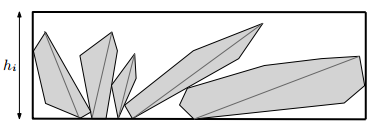
\includegraphics[scale=0.8]{resources/fig1.PNG}
    \caption{Primer pakovanja poligona iz iste visinskoj klasi}
    \label{fig1}
\end{figure}

\begin{lem}
    Povr\v{s}ina kontejnera $B_{i}$ formiranog na gore opisani na\v{c}in zadovoljava: $$area(P_{i}) \leq 2/\alpha \cdot \sum_{p \in P_{i}}{area(p) + 2h_{i} \cdot max_{p \in P_{i}}{width(p)}}$$
\end{lem}


\subsection{Generisanje i pakovanje mini-kontejnera}
\label{subsec:Korak2}

Primenom koraka opisanog u delu \ref{subsec:Korak1} za sve visinske klase dobijamo kolekciju kontejnera $B_{i}$ razli\v{c}itih du\v{z}ina $l_{i}$. Svaki kontejner sadr\v{z}i sve poligone iz visinske klase $P_{i}$. Zamenjujemo svaki kontejner $B_{i}$ mini-kontejnerima jednakih du\v{z}ina na slede\'c{}i na\v{c}in: Neka je $w_{max}$ maksimalna du\v{z}ina poligona iz $P$. Prvo, particioni\v{s}emo $B_{i}$ u \emph{kutije} du\v{z}ine $cw_{max}$ (vrednost za $c$ \'c{}e biti odredjena kasnije) i visine $h_{i}$ \footnote{Osim poslednje kutije, koja mo\v{z}e da ima du\v{z}inu manju od $w_{max}$.}. Sada je potrebno podeliti svaki poligon $p \in P$ u kutiju $b$ koja sadr\v{z}i njegovu najlevlje teme \footnote{Ako najlevlje teme le\v{z}i na granici izmedju dve kutije, dodeljujemo ga desnoj.}. Sada generi\v{s}emo mini-kontejner za svaku kutiju $b$ tako \v{s}to pro\v{s}irujemo $b$ udesno sve dok njena \v{s}irina ne postane ta\v{c}no $(c+1)w_{max}$. Dobijamo kolekciju $\overline{R_{i}}$ od najvi\v{s}e $l_{i}/(cw_{max}) + 1$ mini-kontejnera gde svaki ima istu du\v{z}inu i visinu. Stoga:
$$\sum_{b \in \overline{R_{i}}}{area(b)} \leq (1 + 1/c) \cdot area(B_{i}) + (c+1)w_{max}h_{i}$$

Neka je $\overline{R} = \cup{\overline{R_{i}}}$ kolekcija svih mini-kontejnera dobijenih iznad. Nala\v{z}enje kontejnera za $R$ se obavlja trivijalno bez gubitka povr\v{s}ine postavljanjem mini-kontejnera jedan na drugi \footnote{Ovo je mogu\'c{}e jer svi mini-kontejneri imaju istu du\v{z}inu.}. Tako formiramo kontejner $B$.

\begin{thm}
    Neka je $P$ skup konveksnih poligona u ravni sa ukupnim brojem temena $n$. Mo\v{z}emo spakovati $P$ za vreme $O(n\log{}n)$ u kontejner $B$ koji je pravougaonik sa stranicama paralelnim koordinatnim osama takav da povr\v{s}ina $B$, u oznaci $area(B)$, zadovoljava uslov: $$area(B) \leq 17.45 \cdot OPT$$ gde je $OPT$ povr\v{s}ina optimalnog pravougaonog kontejnera za $P$. 
\end{thm}

\section{Konveksni kontejneri}
\label{sec:Konveksni}


\addcontentsline{toc}{section}{Literatura}
\appendix
\bibliography{literatura}
\bibliographystyle{plain}

%\appendix
%\section{Dodatak}


\end{document}
